\chapter{Grafteori}
Dette kapitel har til formål at beskrive og redegøre for forskellige grafer og de vigtigste elementer i grafteori. 
Grafer kan bruges til mange ting, blandt andet kortlægning af veje i en by, kloaksystemer og forskellige kredsløb.
En graf defineres således: 
\begin{defn}
En graf G = (V,E) består af V, et ikke tomt antal knuder, og E, et antal kanter.
Hver kant har enten en eller to knuder, som den er forbundet til, hvilket kaldes grafens endepunkter.
En kant siges at forbinde dens endepunkter. Dette kaldes en simpel graf.

\end{defn}
\noindent En kant repræsenteres ved en linje mellem to knuder, og knuder repræsenteres ved et punkt.
\begin{figure}[h]
\centering
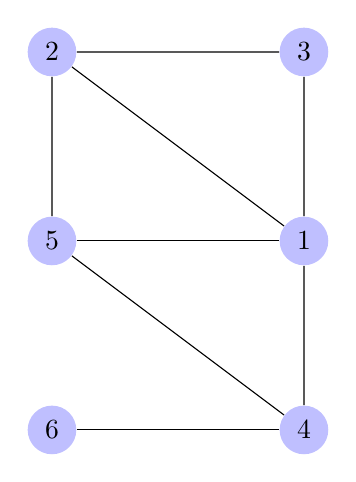
\begin{tikzpicture}
[scale=.8,auto=left,every node/.style={circle,fill=blue!25}]
  \node (n6) at (2,3) {6};
  \node (n4) at (6,3)  {4};
  \node (n5) at (2,6)  {5};
  \node (n1) at (6,6) {1};
  \node (n2) at (2,9)  {2};
  \node (n3) at (6,9)  {3};
  \foreach \from/\to in {n6/n4,n4/n5,n5/n1,n1/n2,n2/n5,n2/n3,n3/n1,n1/n4}
    \draw (\from) -- (\to);
    
\end{tikzpicture}
\caption{Et eksempel på en simpel graf} \label{simpel_graf}
\end{figure}
\\ I figur \ref{simpel_graf} kan der ses en simpel graf med 6 knuder og 8 kanter.
